%%%% début de la page
\teteSndCorp


%%%% titre
%\nomPrenomClasse
\numeroActivite{3}
\titreTP{Identifier des solides et des liquides}

%%%% Contexte 1
\begin{contexte}
  Pour pouvoir identifier des espèces chimiques, on peut utiliser trois méthodes :
  \begin{listePoints}
    \item \important{Mesurer des propriétés physiques} et les comparer à des valeurs de références.
    \item \important{Réaliser des tests chimiques.}
    \item \important{Réaliser une chromatographie sur couche mince (CCM).}
  \end{listePoints}
  Aujourd'hui on va s'intéresser aux deux premières méthodes d'identification.
\end{contexte}


\begin{importants}  
  On cherche à déterminer expérimentalement, avec la plus grande précision possible, la masse volumique d’échantillons métalliques mis à votre disposition.
  
  \hspace{8pt} \problematique{S'agit-il d’aluminium, de cuivre, de zinc ou de fer ?}
\end{importants}

\question{
  Rappeler la relation qui permet de calculer la masse volumique d'un échantillon de matière de masse $m$ et de volume $V$.
}{
  \begin{equation*}
    \rho = \dfrac{m}{V}
  \end{equation*}
}{2}

\begin{doc}{Propriétés physiques de quelques métaux}{doc:TP3_proprietes_metaux}
  \centering
  \begin{tableau}{|c |c |c |}
    Métal
    & Aspect à $T = \qty{20}{\degreeCelsius}$ 
    & Masse volumique (\unit{\g/\cubic\cm}) \\
    %
    Aluminium & Solide gris brillant   & \num{2,700} \\
    Cuivre    & Solide orange brillant & \num{8,960} \\
    Zinc      & Solide gris sombre     & \num{7,150} \\
    Fer       & Solide gris brillant   & \num{7,860}
  \end{tableau}
\end{doc}

\begin{doc}{Volume d'un parallélépipède rectangle}{doc:TP3_volume parallelepipede}
  \begin{multicols}{2}
    Pour calculer le volume d'un parallélépipède rectangle de longueur $L$, de profondeur $p$ et d’épaisseur $e$, on utilise la relation suivante :
    \begin{equation*}
      V = L \times p \times e
    \end{equation*}

    \centering
    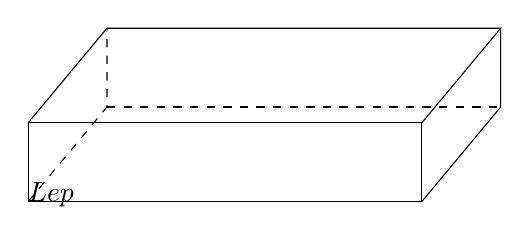
\begin{tikzpicture}
      % Parallelepipede
      \draw (0,0)--(5,0)--(5,1)--(0,1)--(0,0); % face
      \draw (0,1)--(1,2.2)--(6,2.2)--(5,1); % haut
      \draw (5,0)--(6,1.2)--(6,2.2); % côté
      % Perspective
      \draw[dashed] (0,0)--(1,1.2)--(1,2.2); % côté
      \draw[dashed] (1,1.2)--(6,1.2); % fond
      % Legendes
      \tkzVecteur(0)[5](-0.25){$L$}[below]*
      \tkzVecteur(-0.25)(0)[1]{$e$}[left]*
      \tkzVecteur(5.25)[1](-0.1)[1.2]{$p$}[right]*
    \end{tikzpicture}
  \end{multicols}
  Si $L$, $p$ et $e$ sont mesurées en \unit{\cm},
  le résultat s’exprimera en \unit{\cubic\cm}.
\end{doc}

\mesure Mesurer la masse volumique d'un échantillon à l'aide du matériel disponible.

\question{
  En utilisant le document~\ref{doc:TP3_proprietes_metaux}, déterminer la nature de l'échantillon.
}{
  On a mesuré un volume $V = 10,0 \times 2,0 \times \qty{0.2}{\centi\m\cubed} = \qty{4,0}{\centi\m\cubed}$ et une masse $m = \qty{34,0}{\g}$.
  L'échantillon a donc une masse volumique 
  \begin{equation*}  
    \rho
    = \dfrac{30,0}{4,0}\unit{\g/\cubic\centi\m}
    = \qty{7,5}{\g/\cubic\centi\m}
  \end{equation*}

  Comme l'échantillon est brillant et gris, on en déduit qu'on a du fer.
}{2}



%%%% Contexte 2
\begin{importants}
  Les eaux minérales sont des mélanges homogène contenant plusieurs ions de nature et de masses différentes.
  Les eaux minérales sont en général impropre à une consommation régulière, mais elles peuvent servir dans des régimes spécifiques.
  
  \hspace{8pt} \problematique{Comment déterminer les ions présents dans des eaux minérales ?}
\end{importants}



%%%% documents
\begin{doc}{Composition de trois eaux minérales}{doc:TP3_composition_eau}
  \begin{multicols}{3}
    \centering
    \important{Vichy St Yorre} \\ \vspace*{-20pt}
    \begin{tableau}{l | r}
      \SetCell[c=2]{c} Minéralisation : \unit{\mg} pour \qty{1}{\litre} \\
      \ionBicarbonate & \num{4368} \\
      \ionChlorure    & \num{322}  \\
      \ionSodium      & \num{1708} \\
      \ionSulfate     & \num{174}  \\
      \ionPotassium   & \num{110}  \\
      \ionCalcium     & \num{90}   \\
      \ionFluorure    & \num{1}    \\
      \ionMagnesium   & \num{11}   \\
    \end{tableau}

    %
    \important{Mont Roucous} \\ \vspace*{-20pt}
    \begin{tableau}{l | r}
      \SetCell[c=2]{c} Minéralisation : \unit{\mg} pour \qty{1}{\litre} \\
      \ionBicarbonate & \num{1} \\
      \ionChlorure    & \num{2}  \\
      \ionSodium      & \num{3,2}  \\
      \ionSulfate     & \num{6,9}  \\
      \ionFluorure    & < \num{0,1}  \\
      \ionCalcium     & \num{2,7}  \\
      \ionNitrate     & \num{1,8}  \\
      \ionMagnesium   & \num{0,3}  \\
    \end{tableau}
    
    %
    \important{Cristalline} \\ \vspace*{-20pt}
    \begin{tableau}{l | r}
      \SetCell[c=2]{c} Minéralisation : \unit{\mg} pour \qty{1}{\litre} \\
      \ionBicarbonate & \num{228} \\
      \ionChlorure    & \num{15}    \\
      \ionSodium      & \num{8,4}  \\
      \ionSulfate     & \num{11}  \\
      \ionPotassium   & \num{2,3}     \\
      \ionCalcium     & \num{549}   \\
      \ionNitrate     & < \num{1}   \\
      \ionMagnesium   & \num{6,9}   \\
    \end{tableau}

    %
    % \important{Volvic\vphantom{p}} \\
    % \begin{tableau}{l | r}
    %   \SetCell[c=2]{c} Minéralisation : \unit{\mg} pour \qty{1}{\litre} \\
    %   \ionBicarbonate & \num{65,3} \\
    %   \ionChlorure    & \num{8,4}  \\
    %   \ionSodium      & \num{9,4}  \\
    %   \ionSulfate     & \num{6,9}  \\
    %   \ionPotassium   & \num{5,7}  \\
    %   \ionCalcium     & \num{9,9}  \\
    %   \ionNitrate     & \num{6,3}  \\
    %   \ionMagnesium   & \num{6,1}  \\
    % \end{tableau}
    % 
    % %
    % \important{Hépar} \\
    % \begin{tableau}{l | r}
    %   \SetCell[c=2]{c} Minéralisation : \unit{\mg} pour \qty{1}{\litre} \\
    %   \ionBicarbonate & \num{383,7} \\
    %   \ionChlorure    & \num{11}    \\
    %   \ionSodium      & \num{14,2}  \\
    %   \ionSulfate     & \num{1479}  \\
    %   \ionPotassium   & \num{4}     \\
    %   \ionCalcium     & \num{549}   \\
    %   \ionNitrate     & \num{4,3}   \\
    %   \ionMagnesium   & \num{119}   \\
    % \end{tableau}
  \end{multicols}
\end{doc}


%%%%
\begin{doc}{Tests caractéristiques de certains ions}{doc:TP3_tests_ions}
  \begin{center}
    \begin{tableau}{| c | c | c |}
      Ion à tester &
      Réactif utilisé &
      Résultat du test positif \\
      %
      \ionChlorure &
      Solution de nitrate d'argent &
      Précipité blanc, noircit* \\
      %
      \ionSulfate &
      Solution de chlorure de baryum &
      Précipité blanc \\
      %
      \ionCalcium &
      Solution d'oxalate d'ammonium &
      Précipité blanc \\
      %
      \ionMagnesium &
      Solution d'hydroxyde de sodium &
      Précipité blanc
    \end{tableau}
    
    \bigskip
    * Le précipité blanc noircit à la lumière.
  \end{center}
\end{doc}


%%%%
On a trois béchers (A, B, C) contenant des eaux minérales, que vous voulez identifier.

\mesure
Réaliser le protocole suivant :
\begin{protocole}
  \item Verser dans 4 tubes à essais quelques \unit{\mL} d'eau d'un bécher.
  \item Réaliser un test différent dans chaque tube à essais à l'aide des 4 réactifs.
  \item Noter si un précipité se forme et son abondance dans le tableau suivant ($-$, $+$, $++$, $+++$).
  \item Répéter pour les deux autres bécher.
\end{protocole}

\begin{center}
  \begin{tableau}{|l | c | c | c|}
    Test réalisé & Bécher A & Bécher B & Bécher C \\
    Nitrate d'argent    & & & \\
    Chlorure de baryum  & & & \\
    Oxalate d'ammonium  & & & \\
    Hydroxyde de sodium & & &
  \end{tableau}
\end{center}

\question{
  En utilisant les documents~\ref{doc:TP3_composition_eau} et~\ref{doc:TP3_tests_ions}, donner l'eau minérale contenue dans chaque bécher.
}{
  
}{3}
